
\par{Listing \ref{private_local_memory_kernel} shows the kernel that uses 
    together \emph{private memory} to bring a row from A to 
    on-chip memory(as the previous \emph{kernel} did) and 
    \emph{local memory} to cache an entire column of B for all \emph{work items} 
    in a \emph{work group} to reuse. In 
    this case the amount of \emph{local memory} to use is passed to the kernel
    as the fourth argument. The main idea for this is
    that all \emph{work items} in a \emph{work group} share the same column of 
    B to avoid going into \emph{global memory}.}

\par{As in the previous kernel line \emph{12} shows the copy of elements to 
    \emph{private memory} and line \emph{15} shows the 
    copy of elements from \emph{global memory} to \emph{local memory}. This 
    copies are performed by all the \emph{work items} working as a team inside
    of a \emph{work group}(each \emph{work item} load part of the column). 
    To synchronize all the \emph{work items} in a 
    \emph{work group} and to not have data races we use barriers(provided
    by OpenCL) this way all the \emph{work items} in a \emph{work group}
    are forced to wait for all the \emph{work items} to reach this barriers 
    before resuming execution of the next instruction.}

\par{Figure \ref{RowsCols} shows the results of this kernel for different 
    architectures, not all \emph{work group} dimensions 
    were possible to execute for this \emph{kernel}. For the case of the Xeon 
    and Xeon Phi from 32 \emph{work items} per \emph{work group} 
    the runtime returned error -5, that means that a failure ocurred allocating 
    resources\cite{opencl_error}. {\color{red} TODO:Why?}}

\par{Intel Xeon Phi documentation\cite{opencl_phi} advises against using explicit
    local memory, because the cache system takes care of this automatically, 
    furthermore they explain that specifically for the Xeon Phi
    local memory is allocated in 
    \emph{global memory} anyways and the explicit definition of \emph{local
    memory} causes an overhead in terms of redundant data copy and management.
    This can explain the degradation in performance on the Xeon phi shown in
    figure \ref{phi} in comparison with the previous \emph{kernel}. Figure \ref{xeon}
    shows that in the Xeon there is a reduction in execution time even though
    the same issue should happens on the CPU.}

\begin{figure}[!h]
    \centering
    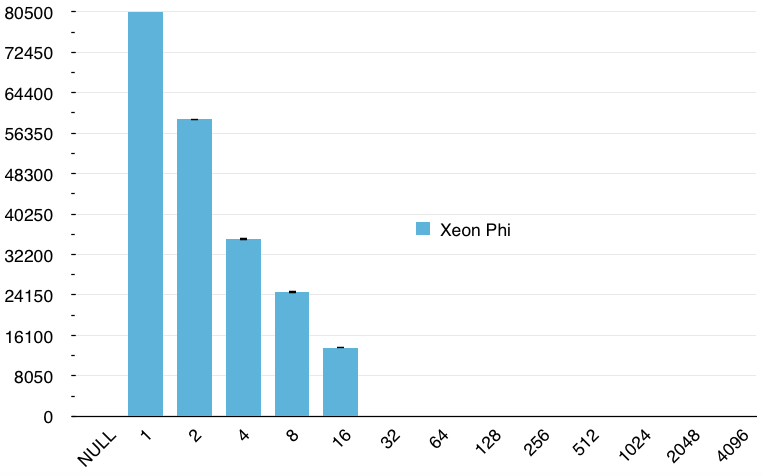
\includegraphics[width=0.49\textwidth]{figures/opt3_phi.png}
    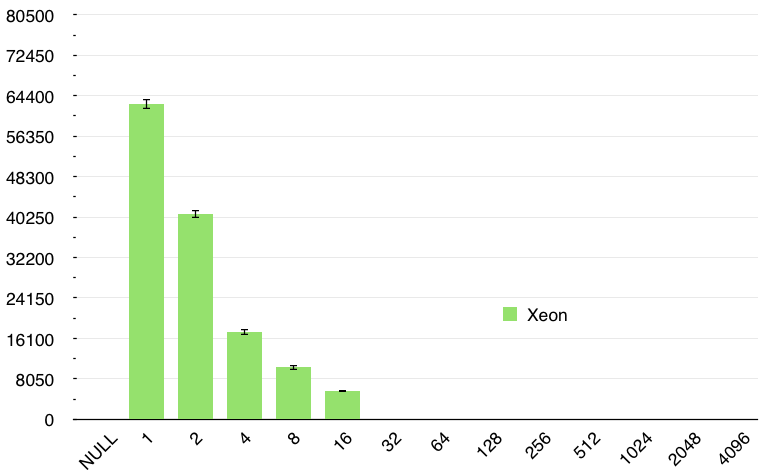
\includegraphics[width=0.49\textwidth]{figures/opt3_cpu.png}
    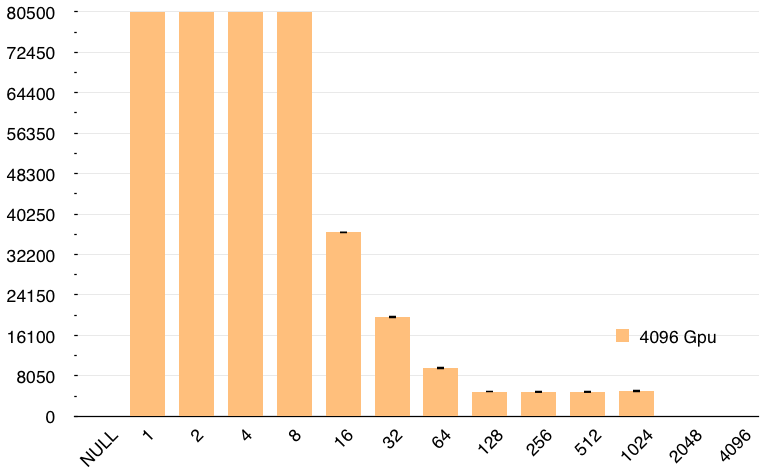
\includegraphics[width=0.49\textwidth]{figures/opt3_gpu.png}
    \caption{Rows and columns optimisation matrix multiplication in different 
            architectures.}
    \label{RowsCols}
\end{figure}

\par{On the Xeon Phi execution it seems to be a trade off, 
    between the the time that takes to execute the loop necesary to 
    copy the elements of B to \emph{local memory}
    (expensive gathering operations with a very poor L1 hit ratio) and the 
    performance achieved in the loop where the kernel executes
    the computation.{\color{red} Maybe vtune shoot of the C kernel}}

\par{Figure \ref{RowsCols} shows that in the GPU while we increment the number of \emph{
    work items} inside of a \emph{work group} the execution time decreases almost
    linearly until the size of 128, because of the utilization of the entire
    width(32) of the warps and the 4 warps available to execute in parallel in
    every SMX. After that the decreasing in time of execution reaches a plateau
     because the resource of every SMX are already full(4 warps per SMX, 32 \emph{
        work items} per warp). Figure
     \ref{gpu} shows that this \emph{kernel} did not improve the performance of 
     the previous \emph{kernel} mainly because the memory access pattern of B
     in the previous \emph{kernel} and B\_local in this \emph{kernel} did not
     change at all, even though we change the algoritm.}

\par{In this case the best time is achived again by the GPU as we can see in 
    figure \ref{RowsColRes}, Also we can notice that the only 
    architectures that is able to take advantage of this optimisation is the 
    Xeon.}

\begin{figure}[!h]
    \centering
    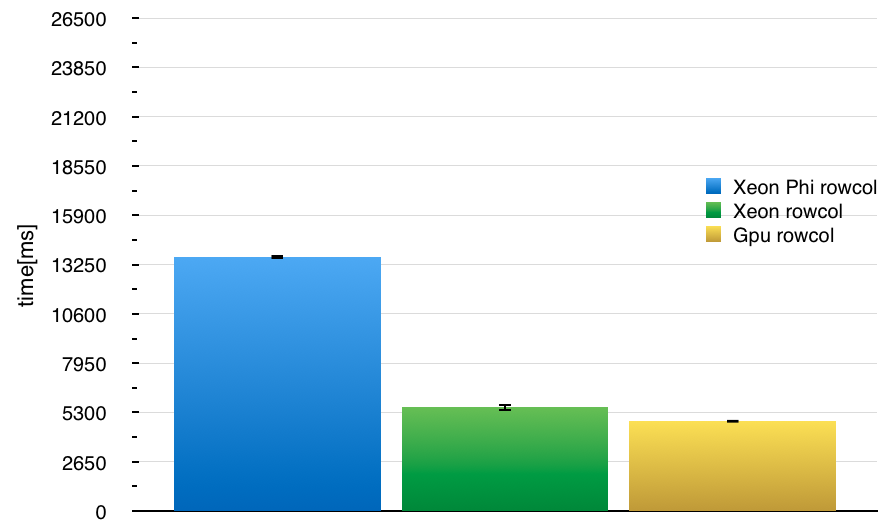
\includegraphics[width=0.49\textwidth]{figures/rowColRes.png}
    \caption{Rows and columns optimisation matrix multiplication best results 
            in different devices.}
    \label{RowsColRes}
\end{figure}

